% EMMA architecture diagram using TikZ (Version 3 - Clean layout)
\documentclass[tikz,border=10pt]{standalone}
\usetikzlibrary{arrows.meta, positioning, calc, shapes.geometric}

\tikzset{
  block/.style={draw, thick, rounded corners, fill=blue!10, minimum width=3.2cm, minimum height=1.6cm, align=center},
  deqblock/.style={draw, thick, rounded corners, fill=green!12, minimum width=3.4cm, minimum height=1.8cm, align=center},
  memory/.style={draw, thick, rounded corners, fill=orange!15, minimum width=3.2cm, minimum height=1.6cm, align=center},
  gate/.style={draw, thick, diamond, aspect=1.6, fill=gray!15, inner sep=1.8pt, align=center},
  io/.style={font=\small},
  label/.style={font=\footnotesize, inner sep=2.5pt, text=black},
  myarrow/.style={-{Latex[length=3.2mm]}, thick},
  optional/.style={dashed, -{Latex[length=3.2mm]}, thick}
}

\begin{document}
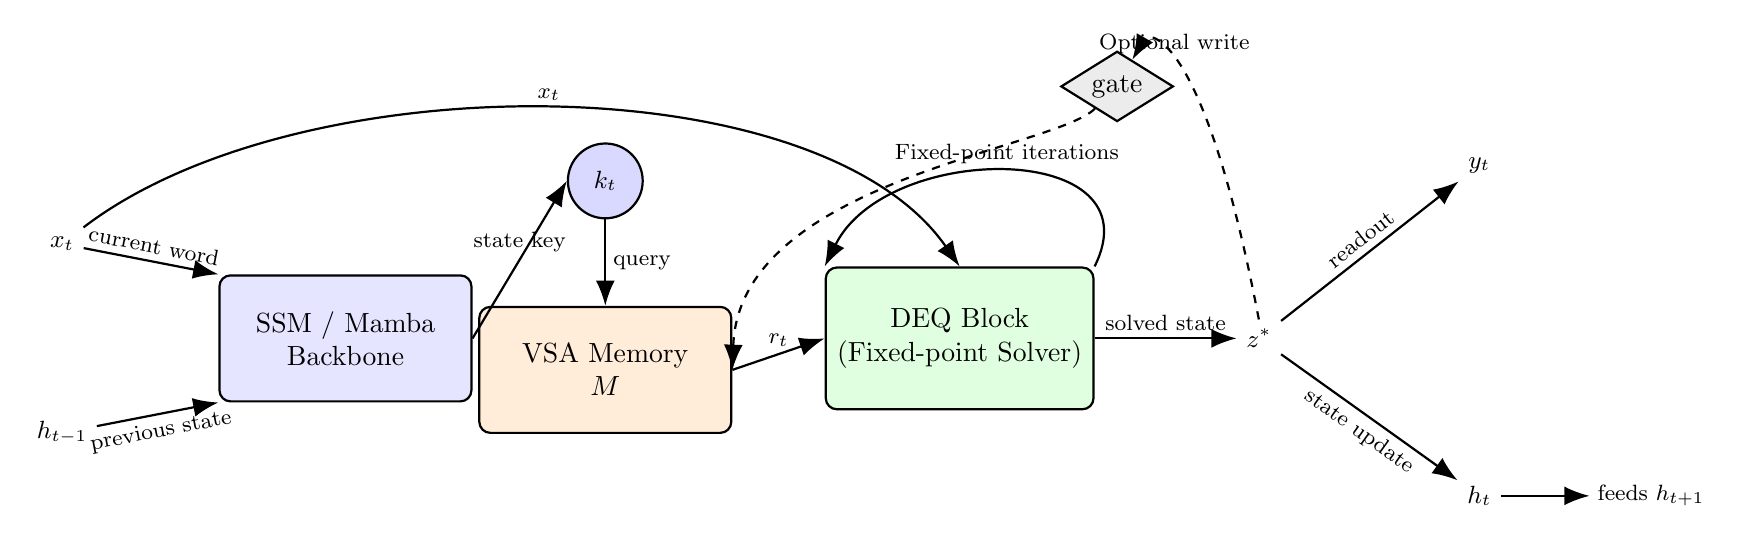
\begin{tikzpicture}[x=1cm, y=1cm]
  % Nodes placed on a grid to avoid overlap
  \node[io] (xt) at (0,0) {$x_t$};
  \node[io] (htm1) at (0,-2.4) {$h_{t-1}$};

  \node[block] (mamba) at (3.6,-1.2) {SSM / Mamba\\Backbone};

  \node[draw, thick, circle, fill=blue!15, minimum size=0.95cm, font=\small] (kt) at (6.9,0.8) {$k_t$};
  \node[memory] (memory) at (6.9,-1.6) {VSA Memory\\$M$};

  \node[deqblock] (deq) at (11.4,-1.2) {DEQ Block\\(Fixed-point Solver)};
  \node[io] (zstar) at (15.2,-1.2) {$z^*$};
  \node[io] (yt) at (18.0,1.0) {$y_t$};
  \node[io] (ht) at (18.0,-3.2) {$h_t$};
  \node[gate] (gate) at (13.4,2.0) {gate};

  % Inputs to SSM / Mamba block
  \draw[myarrow] (xt) -- node[label, above, sloped] {current word} (mamba.north west);
  \draw[myarrow] (htm1) -- node[label, below, sloped] {previous state} (mamba.south west);

  % SSM / Mamba to key and memory
  \draw[myarrow] (mamba.east) -- node[label, above] {state key} (kt.west);
  \draw[myarrow] (kt.south) -- node[label, right] {query} (memory.north);

  % Memory retrieval into DEQ
  \draw[myarrow] (memory.east) -- node[label, above] {$r_t$} (deq.west);

  % Input x_t routed to DEQ
  \draw[myarrow] (xt) .. controls (3.0,2.3) and (9.6,2.3) .. node[label, above] {$x_t$} (deq.north);

  % DEQ fixed-point iterations loop
  \draw[myarrow] (deq.north east) .. controls +(0.8,1.6) and +(0.8,1.6) .. node[label, above] {Fixed-point iterations} (deq.north west);

  % DEQ output to z*
  \draw[myarrow] (deq.east) -- node[label, above] {solved state} (zstar.west);

  % z* to outputs and next state
  \draw[myarrow] (zstar) -- node[label, above, sloped] {readout} (yt);
  \draw[myarrow] (zstar) -- node[label, below, sloped] {state update} (ht);

  % Optional write-back path through a gate
  \draw[optional] (zstar.north) .. controls (14.5,2.7) and (13.8,2.7) .. node[label, above, pos=0.55] {Optional write} (gate);
  \draw[optional] (gate) .. controls (12.6,1.2) and (8.6,0.8) .. (memory.east);

  % Next step hint
  \draw[myarrow] (ht) -- ++(1.4,0) node[label, right] {feeds $h_{t+1}$};
\end{tikzpicture}
\end{document}
